\documentclass{beamer}
\usepackage{multicol}
\usepackage{graphicx}

\graphicspath{{images/}}
\usetheme{CambridgeUS}

\title{The Star Method}
\author[Agbo, Burke, Mako, Vance]{Komi Agbo, Dalton Burke, Nick Mako, James Vance}
\institute[CU Denver]{University of Colorado Denver}
\date{Fall 2019}

\begin{document}
\maketitle

\begin{frame}{Overview}
	\begin{multicols}{2}
	\tableofcontents
	\end{multicols}
\end{frame}

\section{The Problem}
\begin{frame}{Sam's Hauling}
	What do they do?
	\begin{itemize}
		\item Provide roll off dumpsters of various sizes (cans)
		\item Customers 
		\begin{itemize}
			\item Delivery 
			\item Pickup 
			\item Switch 
		\end{itemize}
	\end{itemize}

	\pause
	And how do they do it?
	\begin{itemize}
		\item Resources
			\begin{itemize}
				\item Multiple Trucks
				\item Multiple Landfills
				\item Multiple Storage Yards
				\item Cans
			\end{itemize}
		\item Constraints
			\begin{itemize}
				\item A truck can hold only one can
				\item Truck/Can size compatibility
				\item Customer time preference (AM/PM/None)
			\end{itemize}
	\end{itemize}
\end{frame}

\section{A Small Example}
\begin{frame}{}
	\vspace{-.3cm}
	\begin{center}
	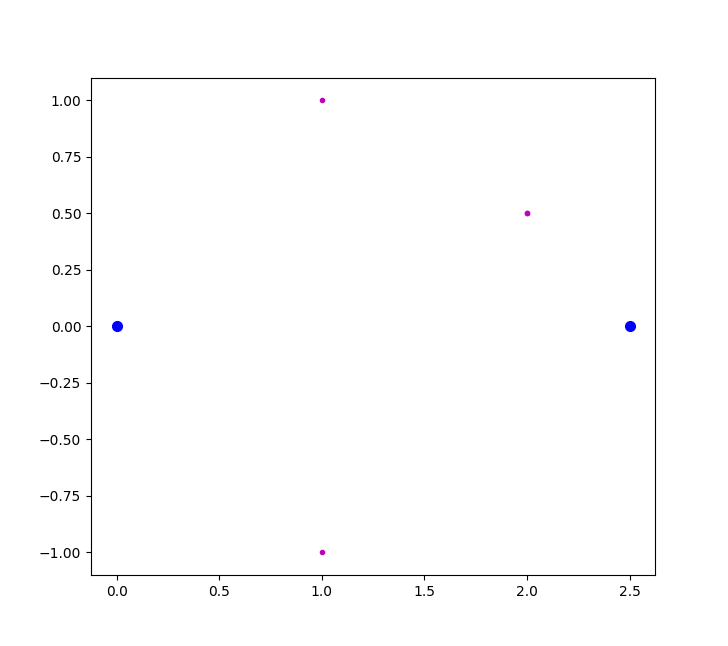
\includegraphics[width=8cm]{landfill_nostar.png}\\
		Landfills (blue), Switches (magenta)
	\end{center}
\end{frame}

\begin{frame}{}
	\vspace{-.3cm}
	\begin{center}
		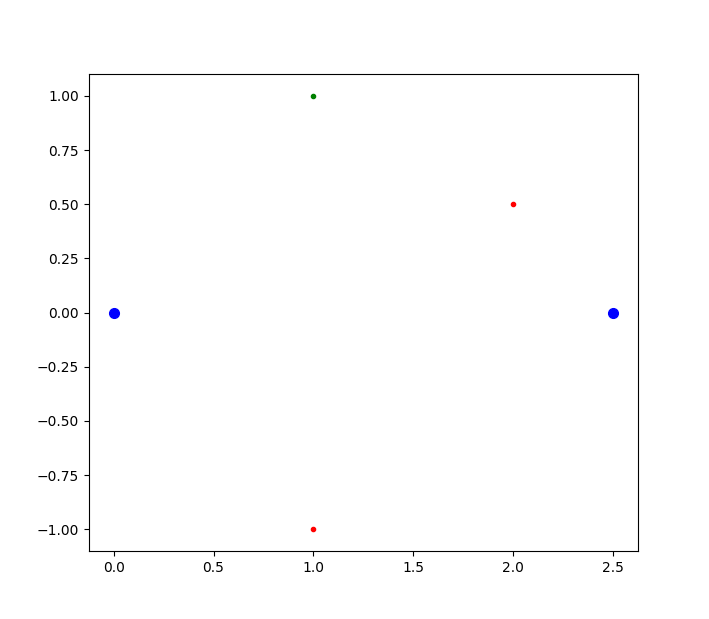
\includegraphics[width=8cm]{landfill_demo.png}\\
		Deliveries (green), Pickups (red)
	\end{center}

\end{frame}

\begin{frame}{How do we find the best triangles?}
	It turns out this problem is very fast to solve, known as a matching problem, and the result is a truly optimal answer.
	\vspace{.5cm}

	In our implementation we used the Munkres library, which has an implementation of the Hungarian Algorithm. This completes the triangle computation in $O(n^3)$ time, the heaviest lifting that we have to do.
\end{frame}

\section{Real Data}
\begin{frame}
	\begin{center}
		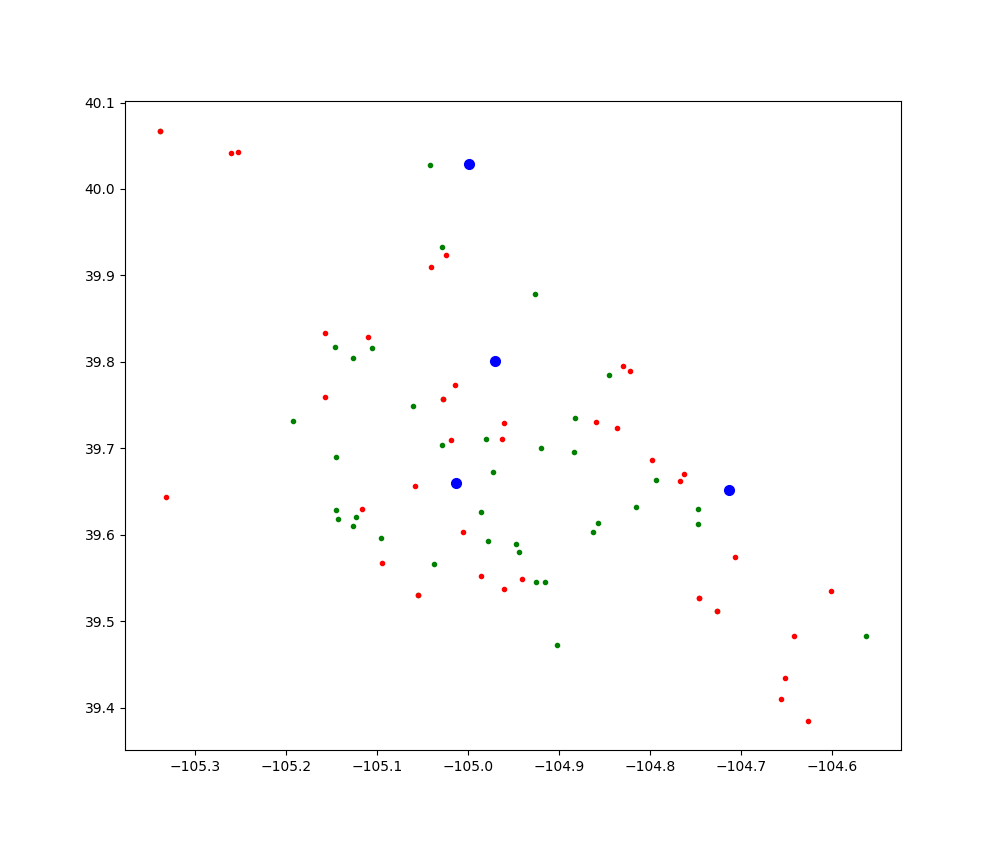
\includegraphics[width=8cm]{empty.png}\\
		Data from a recent day's work
	\end{center}
\end{frame}

\section{Stars}
\begin{frame}
	\begin{center}
		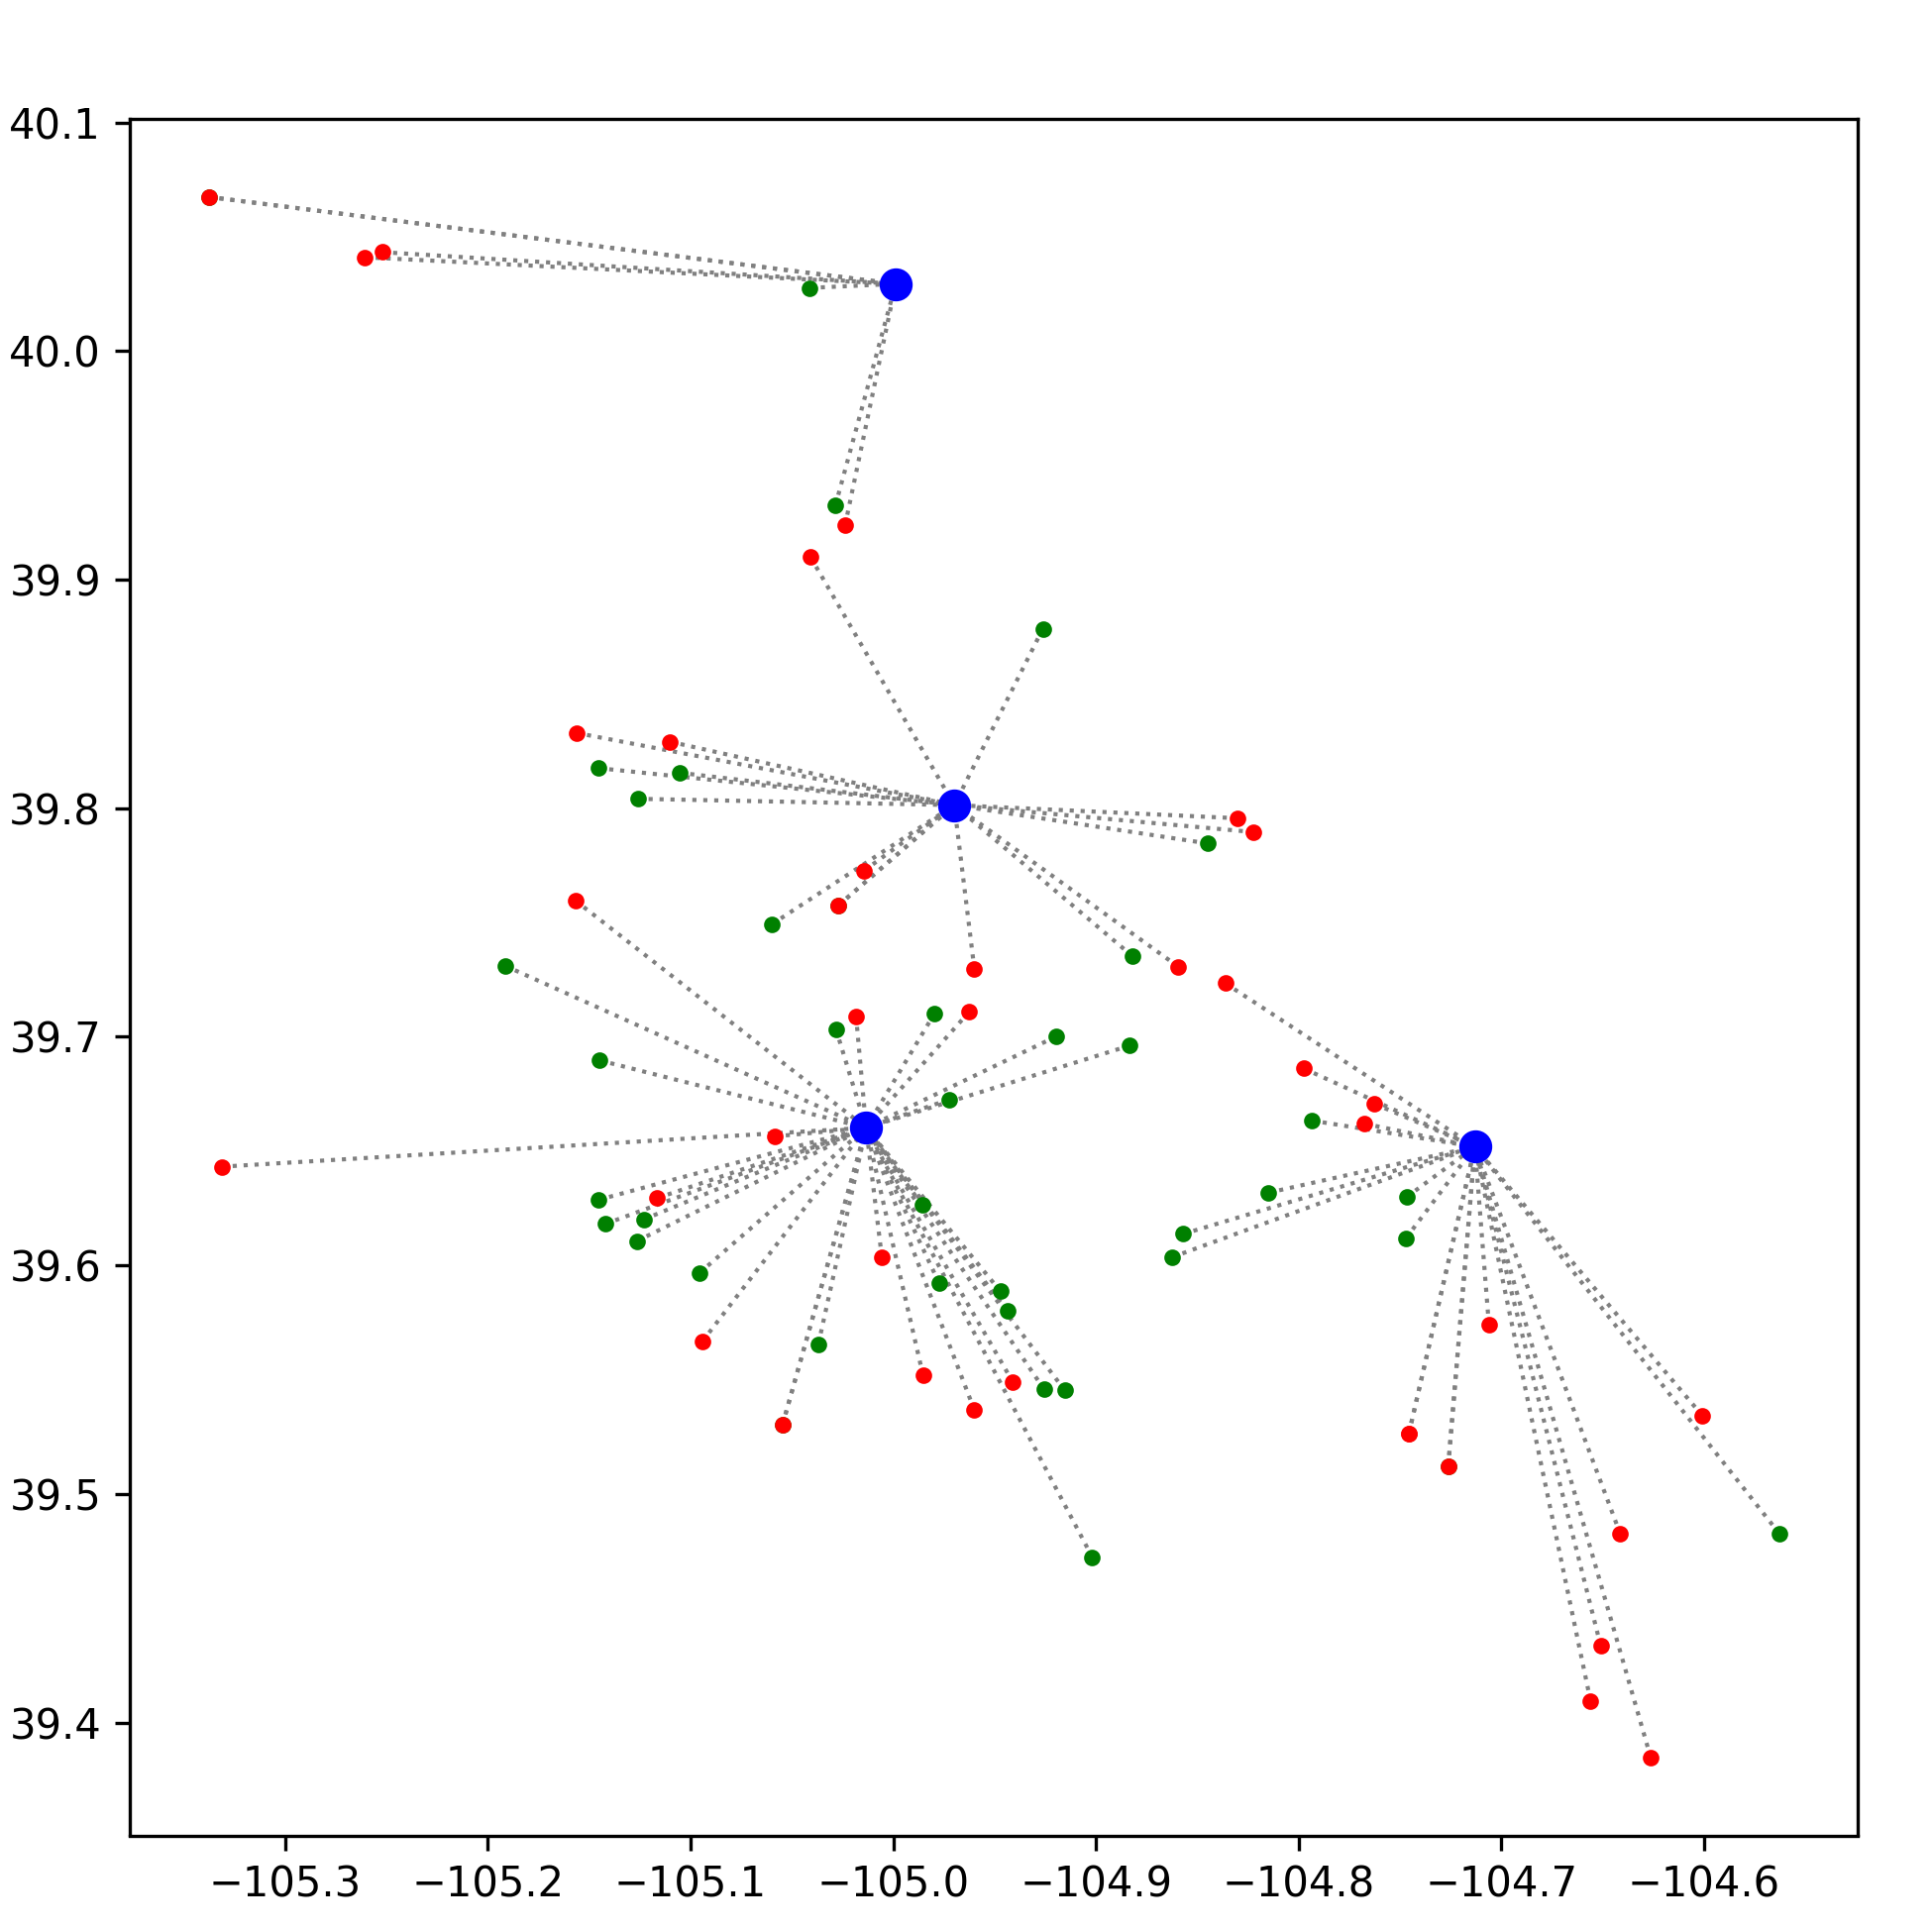
\includegraphics[width=8cm]{stars.png}\\
		Identify the nearest landfill to create \emph{stars}
	\end{center}
\end{frame}

\section{Triangles}
\begin{frame}
	\begin{center}
		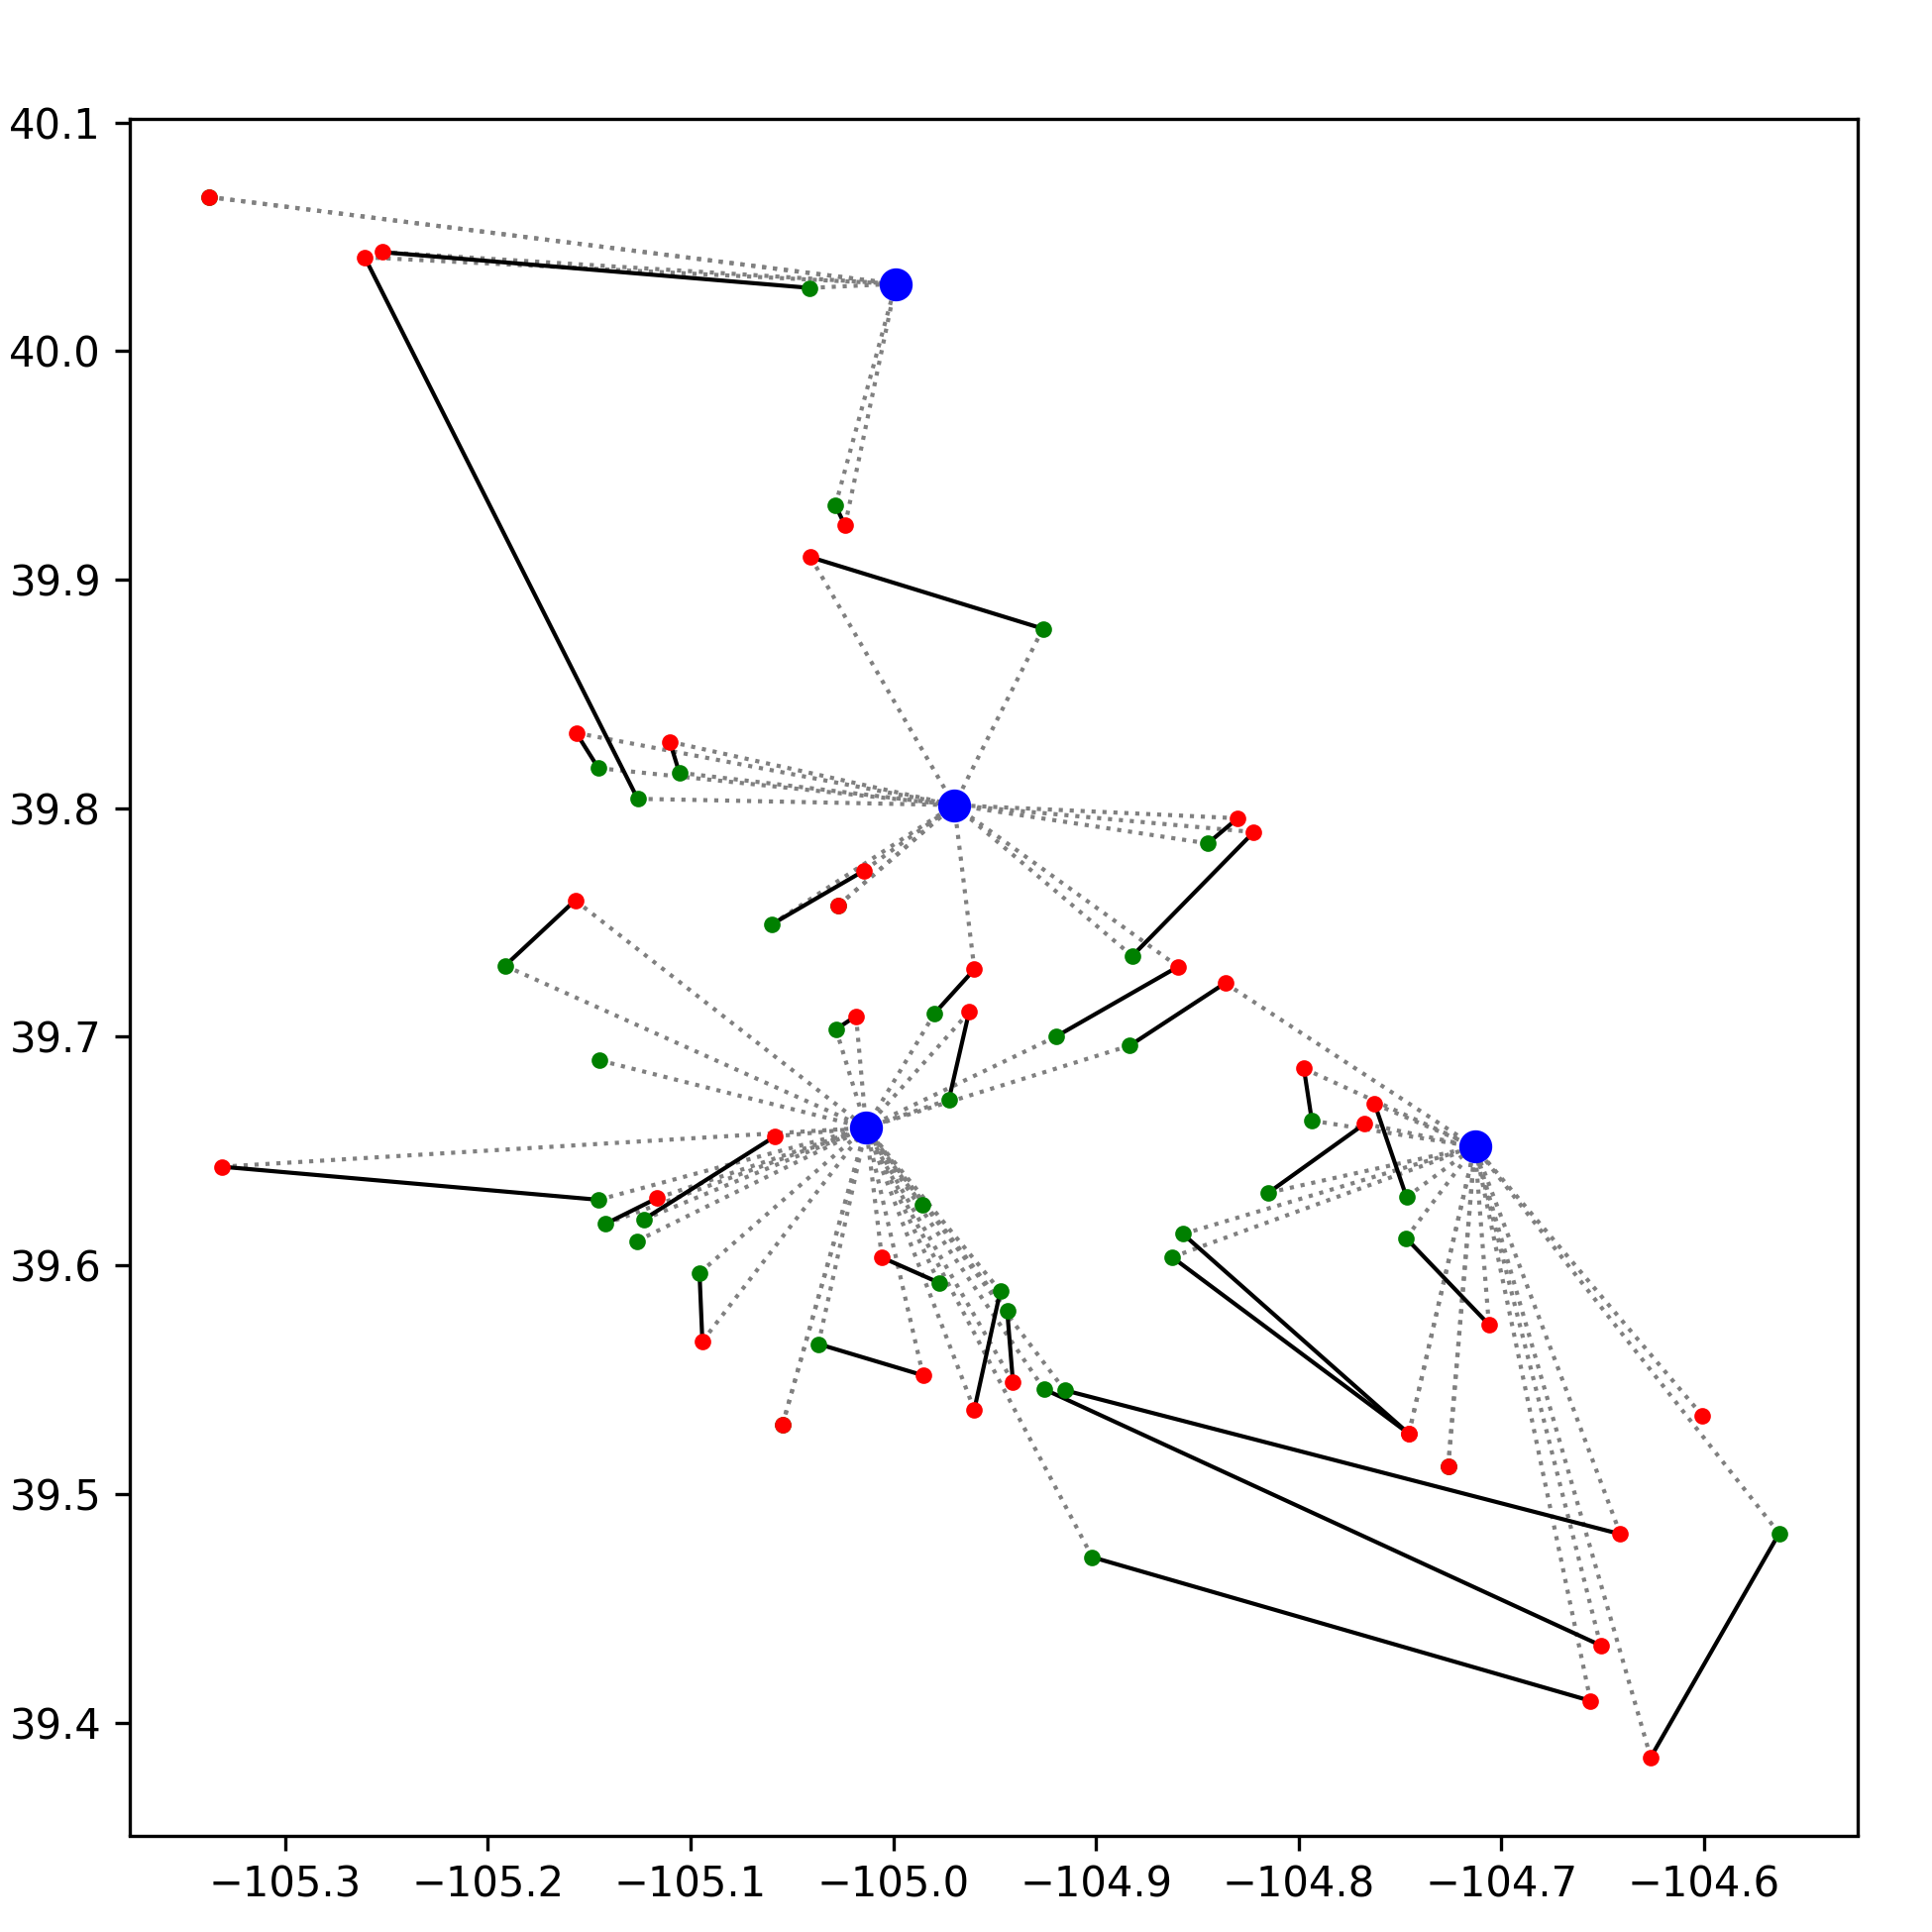
\includegraphics[width=8cm]{triangles.png}\\
		Identify the best set of pairs to create \emph{triangles}
	\end{center}
\end{frame}

\section{Route Building}
\begin{frame}
Now to actually build the routes for the drivers...

\end{frame}


\begin{frame}
The algorithm for assigning the full schedule are as follows:
\begin{enumerate}
\item Receive data for the day and process it into the program.
\item Create pairs with Hungarian algorithm.
\item Assign driver to resolve truck size constraint.
\item Transition to the farthest zone that requires the truck resolving a hard can deficit if applicable.
\item Service all routes within the zone that require the truck and return to 2 if more applicable routes exist in other zones.
\item Finish route as per a normal driver and return to 1 if other truck size constraints exist.
\item Assign next driver to farthest zone with routes.
\item Transition to the zone.
\item If applicable resolve hard can deficits.
\item Assign remaining routes by prioritizing AM/PM constraints and then distance to the main hub.
\item If there are no more routes in the zone return to 6 choosing the next zone with routes remaining.
\item If the driver schedule is full including the transition back to the main hub transition back to the main hub and return to 6.
\item Iterate through the day to resolve any soft can deficits.
\item Output schedules.
\end{enumerate}
\end{frame}

\section{Results} 
\begin{frame}
From an old schedule provided by the client, we ran our algorithm to see how it stacked up to the clients solution \textbf{(comparison pending, will be present in final)}. In the following figures, each color is a driver's route.
\end{frame}

\section{Using it}
\begin{frame}
	New requirements for the customer (file organization)
\end{frame}

\section{Conclusions/Future Work} 
\begin{frame}
There are two things that would make this program better, one, is better data. If given actual driving times, the output would do a much better job of reflecting real world conditions. As of now, we actually can't even test how well it's doing.

The other thing that would make this better is a better pair choice reflecting the transitions that will inevitably need to be taken. Right now, pairs are chosen as if drivers can teleport between landfills. While a vast majority of a drivers time is \emph{not} taking transitions, it still seems like we are losing a bit here. In order to truely take them into account however, it seems like a much more painful implementation than what is presented. 

In the end, having to take the transitions (as opposed to teleporting between landfills) cost the route about 90 minutes, out of 1622, which is around a $5.5\%$ difference. An improvement could only save us about that much. The obvious next step is to find a bound for the difference between teleportation and our output, however, due to time constraints, we leave it unanswered for now.
\end{frame}

\section*{Summary}
\begin{frame}{What we covered}
\begin{multicols}{2}
	\tableofcontents
\end{multicols}
\end{frame}

\end{document}
